\documentclass[12pt]{article}
\usepackage{graphicx}
\usepackage[none]{hyphenat}
\usepackage{graphicx}
\usepackage{listings}
\usepackage[english]{babel}
\usepackage{graphicx}
\usepackage{caption} 
\usepackage{booktabs}
\usepackage{array}
\usepackage{amssymb} % for \because
\usepackage{amsmath}   % for having text in math mode
\usepackage{extarrows} % for Row operations arrows
\usepackage{listings}
\lstset{
  frame=single,
  breaklines=true
}
\usepackage{hyperref}
\usepackage{mathtools}

%Following 2 lines were added to remove the blank page at the beginning
\usepackage{atbegshi}% http://ctan.org/pkg/atbegshi
\AtBeginDocument{\AtBeginShipoutNext{\AtBeginShipoutDiscard}}


%New macro definitions
\newcommand{\mydet}[1]{\ensuremath{\begin{vmatrix}#1\end{vmatrix}}}
\providecommand{\brak}[1]{\ensuremath{\left(#1\right)}}
\providecommand{\sbrak}[1]{\ensuremath{{}\left[#1\right]}}
\providecommand{\norm}[1]{\left\lVert#1\right\rVert}
\providecommand{\abs}[1]{\left\vert#1\right\vert}
\newcommand{\solution}{\noindent \textbf{Solution: }}
\newcommand{\myvec}[1]{\ensuremath{\begin{pmatrix}#1\end{pmatrix}}}
\let\vec\mathbf


\begin{document}

\begin{center}
\title{\textbf{Linear Programming}}
\date{\vspace{-5ex}} %Not to print date automatically
\maketitle
\end{center}
\setcounter{page}{1}

\section{12$^{th}$ Maths - Chapter 12}
This is Problem-1 from Exercise 12.1
\begin{enumerate}
\item Maximize
\begin{align}
	Z = 3x + 4y
\end{align}
subject to the constraints:
\begin{align}
	x+4y \leq 4, \\ 
	x \geq 0, y \geq 0
\end{align}
\solution 
The given problem can be formulated as 
\begin{align}
	\max_{\vec{x}} Z &= \myvec{3 & 4}\vec{x} \\
        \myvec{1 & 4\\
               -1 &0\\
	       0 & -1}\vec{x}\preceq & \myvec{4 \\0\\0}
\end{align}
Solving using cvxpy, we get
\begin{align}
	\max_{\vec{x}} Z &= 12 \\
	\vec{x} &= \myvec{4  \\  0} 
\end{align}
The figure is as shown in Fig\ref{fig:Fig1}
\begin{figure}[!h]
	\begin{center}
		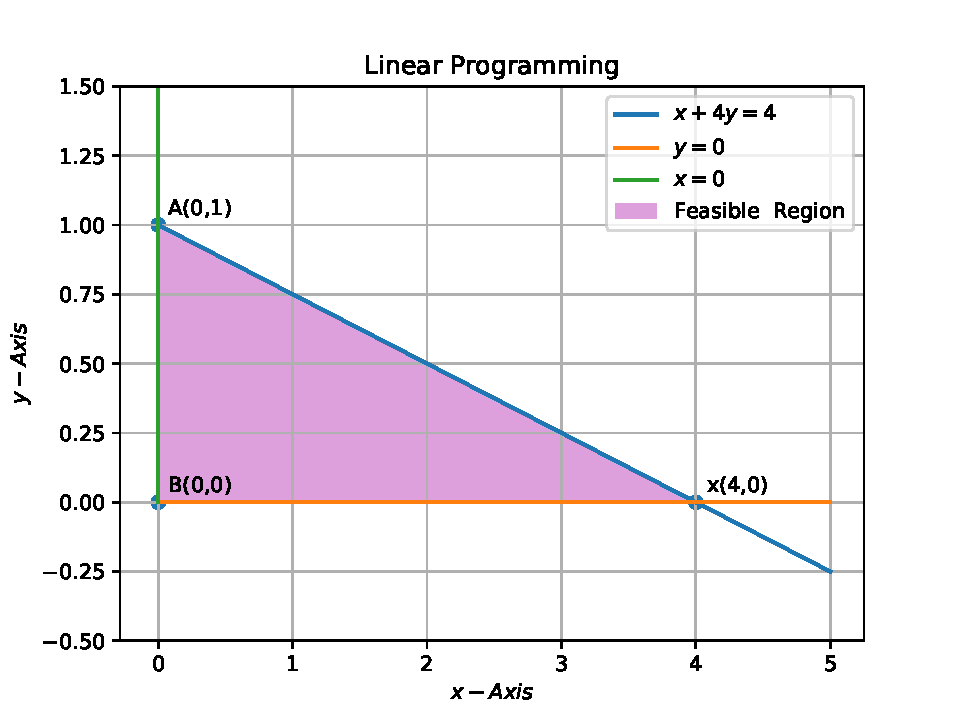
\includegraphics[width=\columnwidth]{figs/problem1.pdf}
	\end{center}
\caption{}
\label{fig:Fig1}
\end{figure}
\end{enumerate}
\end{document}
